\documentclass[12pt,a4paper]{report}
\usepackage[margin=1in]{geometry}
\usepackage[T1]{fontenc}
\usepackage{lmodern,microtype,graphicx,booktabs,float,amsmath,xcolor,hyperref,listings,enumitem}
\hypersetup{colorlinks=true,linkcolor=black,urlcolor=blue,pdftitle={KnightScope Project Report}}
\setlength{\parskip}{0.55em}
\setlength{\parindent}{0pt}
\renewcommand{\arraystretch}{1.16}
\definecolor{codegray}{RGB}{245,245,245}
\lstset{basicstyle=\ttfamily\small,backgroundcolor=\color{codegray},frame=single,breaklines=true}
\begin{document}
\begin{titlepage}
\centering\vspace*{1.8cm}
{\LARGE\textbf{PROJECT REPORT}\par}\vspace{1.1cm}
{\Huge\textbf{KnightScope}\par}\vspace{0.35cm}
{\Large Intelligent Chess Position Analysis Using Classical AI\par}\vspace{1.2cm}
\rule{0.78\textwidth}{0.7pt}\par\vspace{0.7cm}
{\large Submitted for \textbf{Artificial Intelligence with Python}\par}\vspace{0.35cm}
{\large Academic Year 2026\par}\vspace{1.3cm}
\begin{tabular}{rl}
\textbf{Team:} & Deep Knights (4 members)\\
\textbf{Application:} & Interactive chess position analyser\\
\textbf{Implementation:} & Python search engine and interactive web interface\\
\textbf{Submission date:} & 21 November 2026
\end{tabular}
\vfill{\large Department of Computer Science and Engineering\par}
\end{titlepage}
\pagenumbering{roman}
\chapter*{Declaration}\addcontentsline{toc}{chapter}{Declaration}
We declare that KnightScope was developed as a course project by Team Deep Knights. The project implements its own Minimax, Alpha-Beta, Greedy, and Iterative Deepening procedures. The \texttt{python-chess} library is used for board state, legal-move generation, FEN handling, and chess-rule validation. No external chess engine, chess API, neural model, or precomputed engine evaluation is used to select moves.

\chapter*{Abstract}\addcontentsline{toc}{chapter}{Abstract}
KnightScope is a Python-based chess-analysis project with an interactive web demonstration. A user can arrange a position, import a FEN position, set the side to move and search depth, then receive a recommended move, heuristic score, principal variation, and search statistics. The Python implementation contains depth-limited Minimax, Alpha-Beta Pruning, a one-ply Greedy baseline, and Iterative Deepening built from Alpha-Beta searches. Its evaluation function combines material, piece-square values, mobility, centre control, king safety, pawn structure, and bishop-pair information.

The stored experiments cover ten legal chess positions. Alpha-Beta matched Minimax's move and score in all 30 position-depth comparisons while visiting fewer nodes at depths two and three. At depth three, the mean recorded node reduction was 94.11\% and the mean recorded speed-up was 29.31$\times$. Greedy agreed with the depth-three adversarial choice in two of ten cases. The report documents a current limitation: Iterative Deepening checks its budget between completed iterations, so one deep iteration can overrun the requested limit. The report presents design, evidence, limitations, and future work without claiming professional chess-engine strength.

\tableofcontents\listoffigures\listoftables\clearpage\pagenumbering{arabic}
\chapter{Introduction}
Chess is a useful model for adversarial decision-making. Two players act in turn, every state is visible, and one player's advantage is the other's disadvantage. The number of continuations grows rapidly, so a useful program needs a search strategy and a heuristic for positions that cannot be searched to the end of a game.

KnightScope is a position analyser rather than a game-playing service. It accepts a legal position and reports the best move found under a selected search depth and evaluation function. The recommendation is a bounded-search result, not a claim of objectively best chess play.

\section{Objectives}
\begin{enumerate}[label=\arabic*.]
\item Implement classical AI algorithms in a working Python application.
\item Formulate chess analysis as a state-space and adversarial-search problem.
\item Compare methods through recorded execution time, explored nodes, pruning, move choice, and evaluation score.
\item Provide a visual interface for FEN input, analysis, comparison, and explanation.
\end{enumerate}

\chapter{Problem Formulation}
The problem is represented by $\langle S_0,A,Result,Terminal,Utility,H\rangle$.
\begin{table}[H]\centering\caption{KnightScope problem formulation}
\begin{tabular}{p{0.26\textwidth}p{0.64\textwidth}}\toprule
Component & Definition\\\midrule
Initial state $S_0$ & A legal FEN position, including side to move and rule state.\\
Actions $A(s)$ & All legal moves available in state $s$.\\
Transition $Result(s,a)$ & The successor position after legal move $a$.\\
Goal & Select the highest-valued root move under a bounded search model.\\
Terminal test & Checkmate, stalemate, insufficient material, or a claimable draw.\\
Constraints & Chess rules, finite depth, and optional time budget.\\
Heuristic $H(s)$ & White-relative centipawn score with material and positional features.\\\bottomrule
\end{tabular}\end{table}

White maximizes the evaluation and Black minimizes it. For a non-terminal state, depth-limited Minimax is:
\[
V(s,d)=\begin{cases}U(s)&\text{if }s\text{ is terminal}\\H(s)&\text{if }d=0\\
\max_{a\in A(s)}V(Result(s,a),d-1)&\text{if White moves}\\
\min_{a\in A(s)}V(Result(s,a),d-1)&\text{if Black moves.}\end{cases}
\]

\chapter{System Design and Implementation}
\section{Architecture}
The project separates the interface, chess utilities, search engines, evaluation function, benchmark scripts, tests, and documentation. The Python engine package implements search and the analysis package runs experiments and writes CSV files. The public browser interface demonstrates position editing, FEN import/export, board flipping, depth selection, and Alpha-Beta move analysis. This separation lets the same engine functions support the application, automated tests, and experiments.

\begin{table}[H]\centering\caption{Core technology choices}
\begin{tabular}{p{0.30\textwidth}p{0.55\textwidth}}\toprule
Technology & Purpose\\\midrule
Python & Main implementation language\\
HTML, CSS, and JavaScript & Public interactive board and browser demonstration\\
python-chess & Legal moves, board state, FEN validation, and chess rules\\
Plotly and Matplotlib & Interactive and report visualisation\\
Pandas and NumPy & Benchmark tables and aggregation\\
pytest & Automated test suite supplied with the project\\\bottomrule
\end{tabular}\end{table}

\section{Evaluation Function}
The score is white-relative: positive values favour White and negative values favour Black. Terminal positions override ordinary heuristic values. Checkmate receives a large signed score and draws receive zero.
\begin{table}[H]\centering\caption{Evaluation features}\label{tab:eval}
\begin{tabular}{p{0.33\textwidth}p{0.15\textwidth}p{0.38\textwidth}}\toprule
Feature & Weight & Implementation intent\\\midrule
Material & 1.0 & Pawn 100, knight 320, bishop 330, rook 500, queen 900 centipawns.\\
Piece-square tables & 1.0 & Reward useful placement and pawn advancement.\\
Mobility & 0.1 & Difference in legal movement opportunities.\\
Centre control & 0.3 & Occupation or attack of d4, e4, d5, and e5.\\
King safety & 0.5 & Pawn shelter near the king.\\
Pawn structure & 0.25 & Doubled and isolated pawn penalties.\\
Bishop pair & 0.5 & Bonus for two bishops.\\\bottomrule
\end{tabular}\end{table}
The weights are hand-set. The function is interpretable but does not model all chess concepts, so it is an educational heuristic rather than a calibrated engine evaluation.

\chapter{Algorithms}
\section{Minimax}
Minimax explores every legal line to the selected depth. It alternates MAX nodes for White and MIN nodes for Black, then propagates leaf evaluations to the root. It provides the exact result for its chosen depth and heuristic, but the node count grows quickly with the branching factor.

\section{Alpha-Beta Pruning}
Alpha-Beta retains Minimax's result while maintaining $\alpha$, the best value guaranteed to MAX, and $\beta$, the best value allowed by MIN. When $\beta\leq\alpha$, remaining sibling moves cannot affect the root decision and are skipped. KnightScope orders tactical moves before quieter moves to make cutoffs more likely. The implementation counts explored nodes and skipped sibling moves.

\section{Greedy Best-First Baseline}
Greedy evaluates every immediate successor and selects the best one-ply score for the current side. It is a baseline rather than an equivalent adversarial search: it does not model an opponent reply and cannot reliably identify tactical refutations.

\section{Iterative Deepening}
Iterative Deepening runs Alpha-Beta at depth 1, then 2, and so on, preserving the result of the last completed search. The present program checks a time budget before and after each full Alpha-Beta iteration. It does not interrupt a search that is already running, which is a known limitation.

\chapter{User Interface and Demonstration}
The public interface lets the user move, add, and remove pieces; choose a side to move; change castling flags; flip the board; load a FEN; and run Alpha-Beta analysis at depth one to three. The demonstration website is available at \url{https://knightscope-classic.onrender.com}. The source repository is \url{https://github.com/HaMaMi-1/KnightScope}.
\begin{figure}[H]\centering
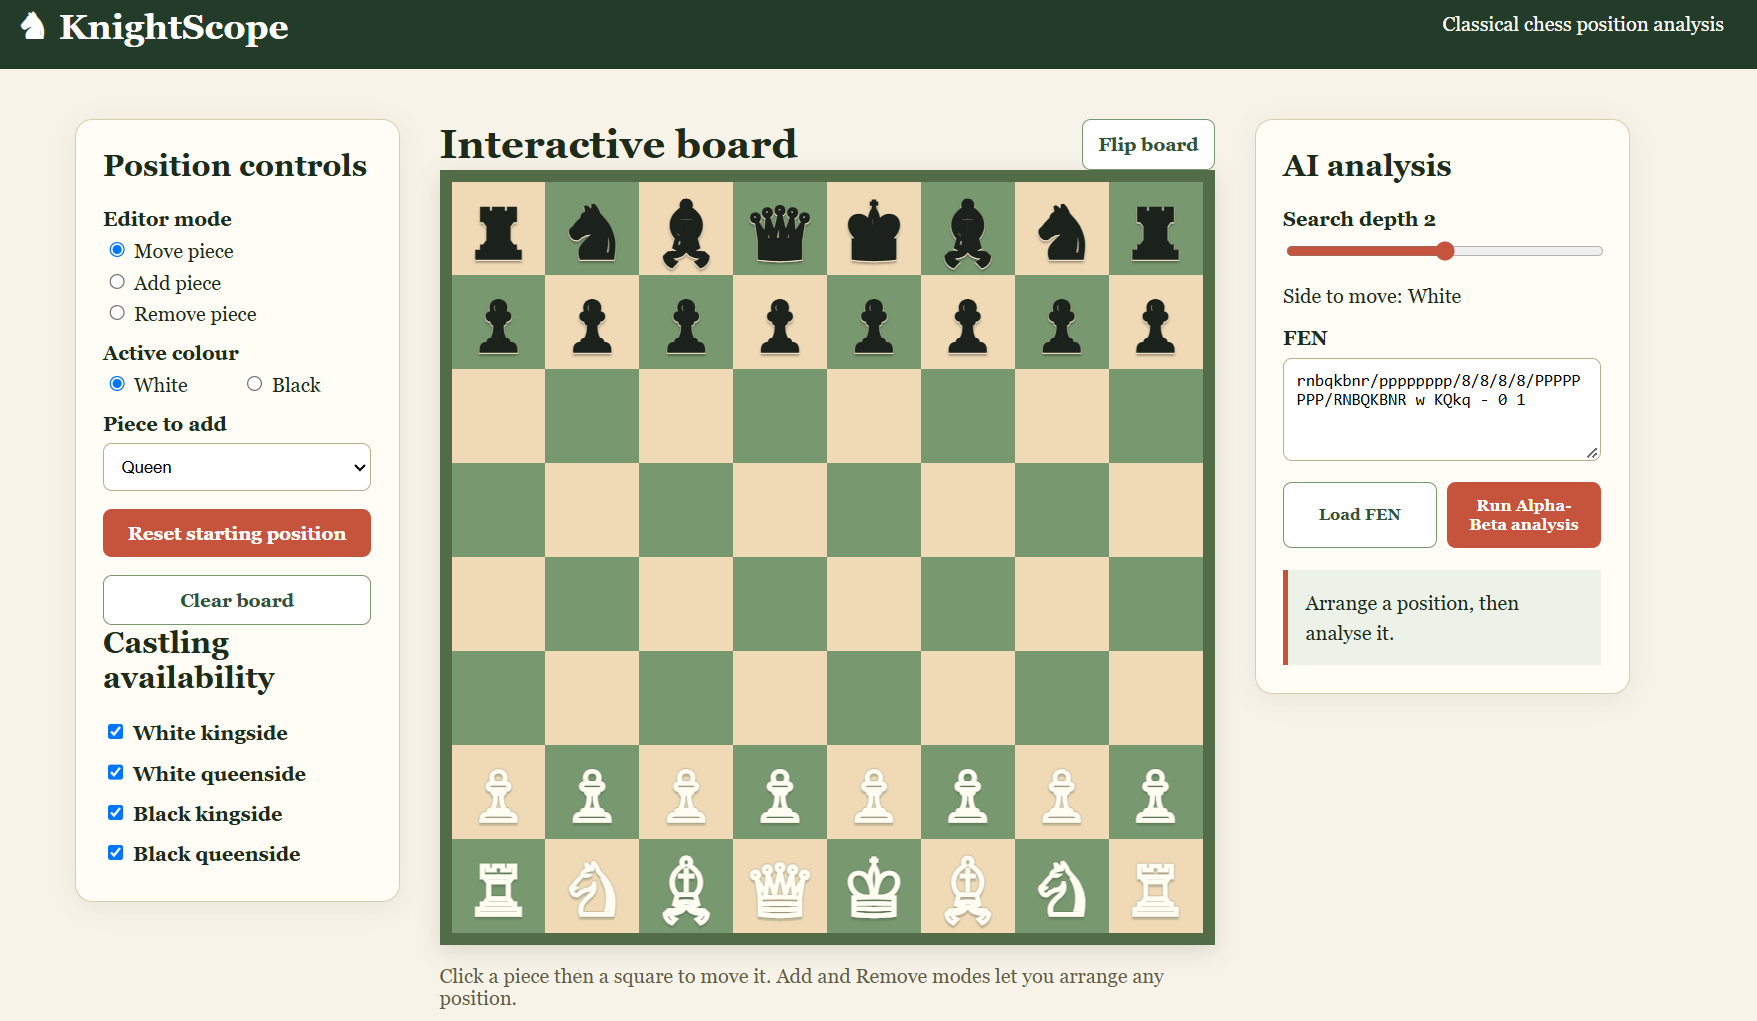
\includegraphics[width=0.92\textwidth]{images/initial-position.png}
\caption{Interactive board in its starting configuration}\end{figure}
\begin{figure}[H]\centering
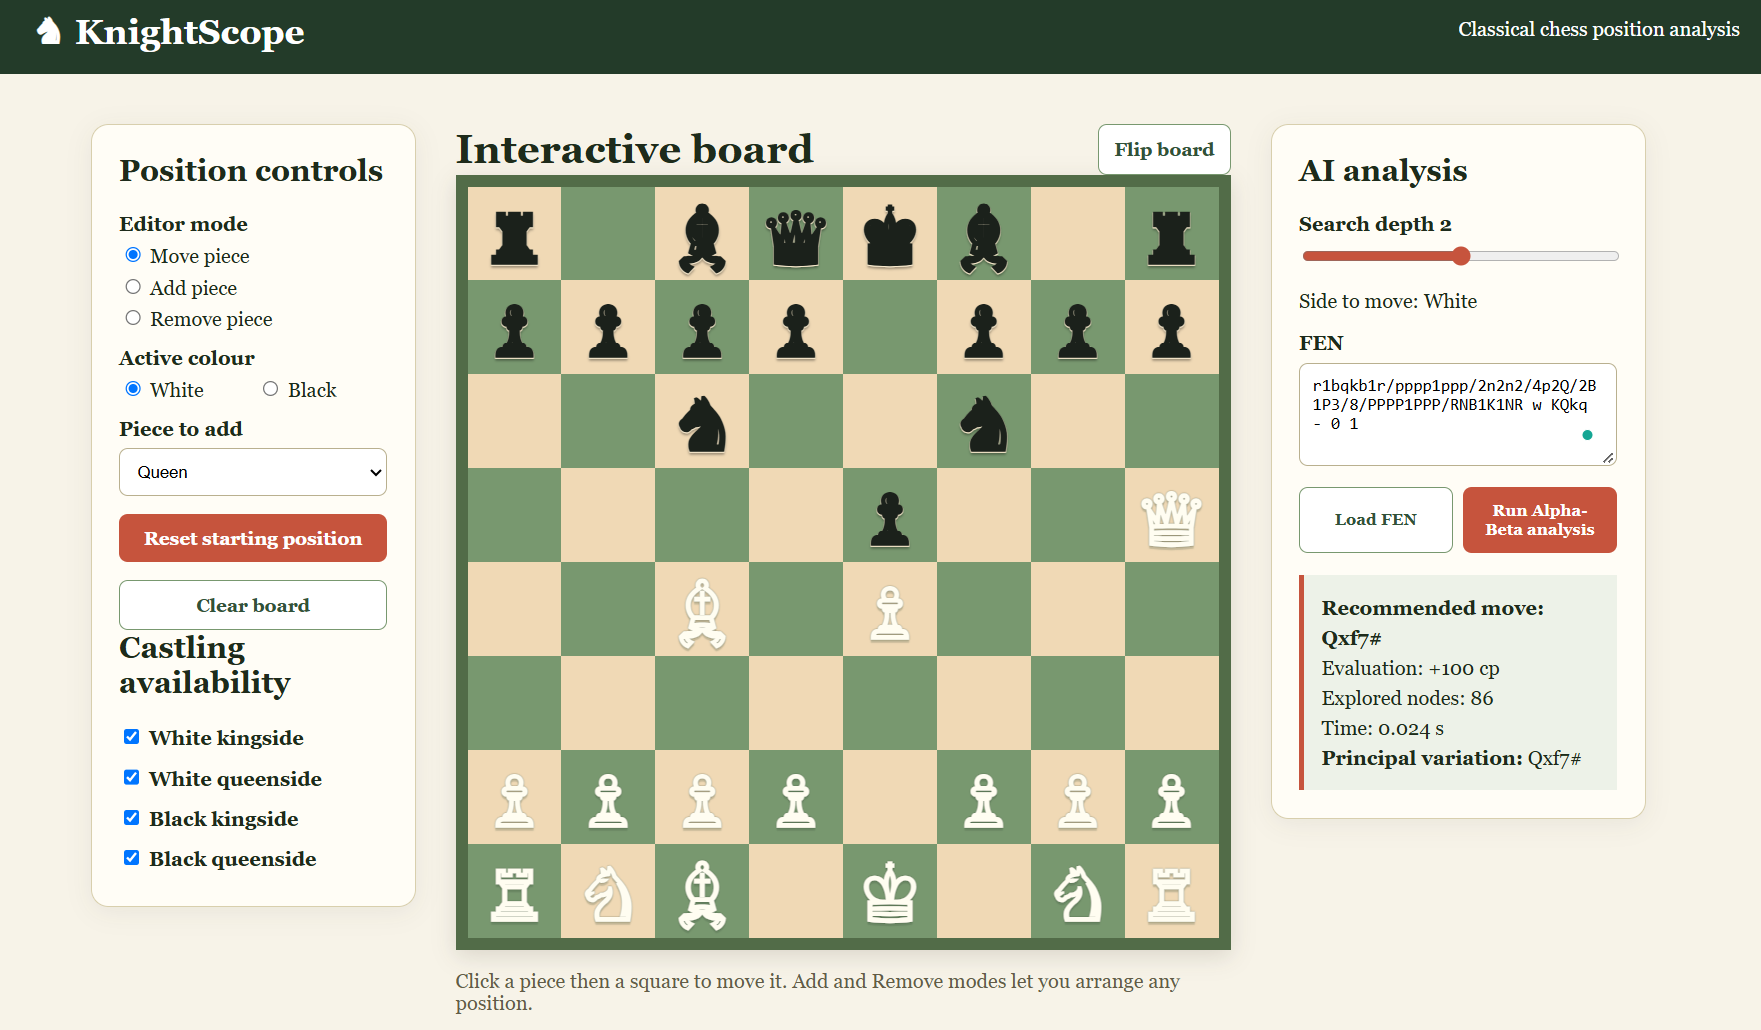
\includegraphics[width=0.92\textwidth]{images/forced-mate.png}
\caption{Forced-mate demonstration: the interface recommends Qxf7\# at depth two}\end{figure}

\section{Representative Interactive Results}
The following screenshots document individual demonstration runs. They are not a controlled depth comparison because each position differs. Their purpose is to show the working editor, side-to-move handling, recommended move, explored-node count, elapsed time, and principal variation.
\begin{figure}[H]\centering
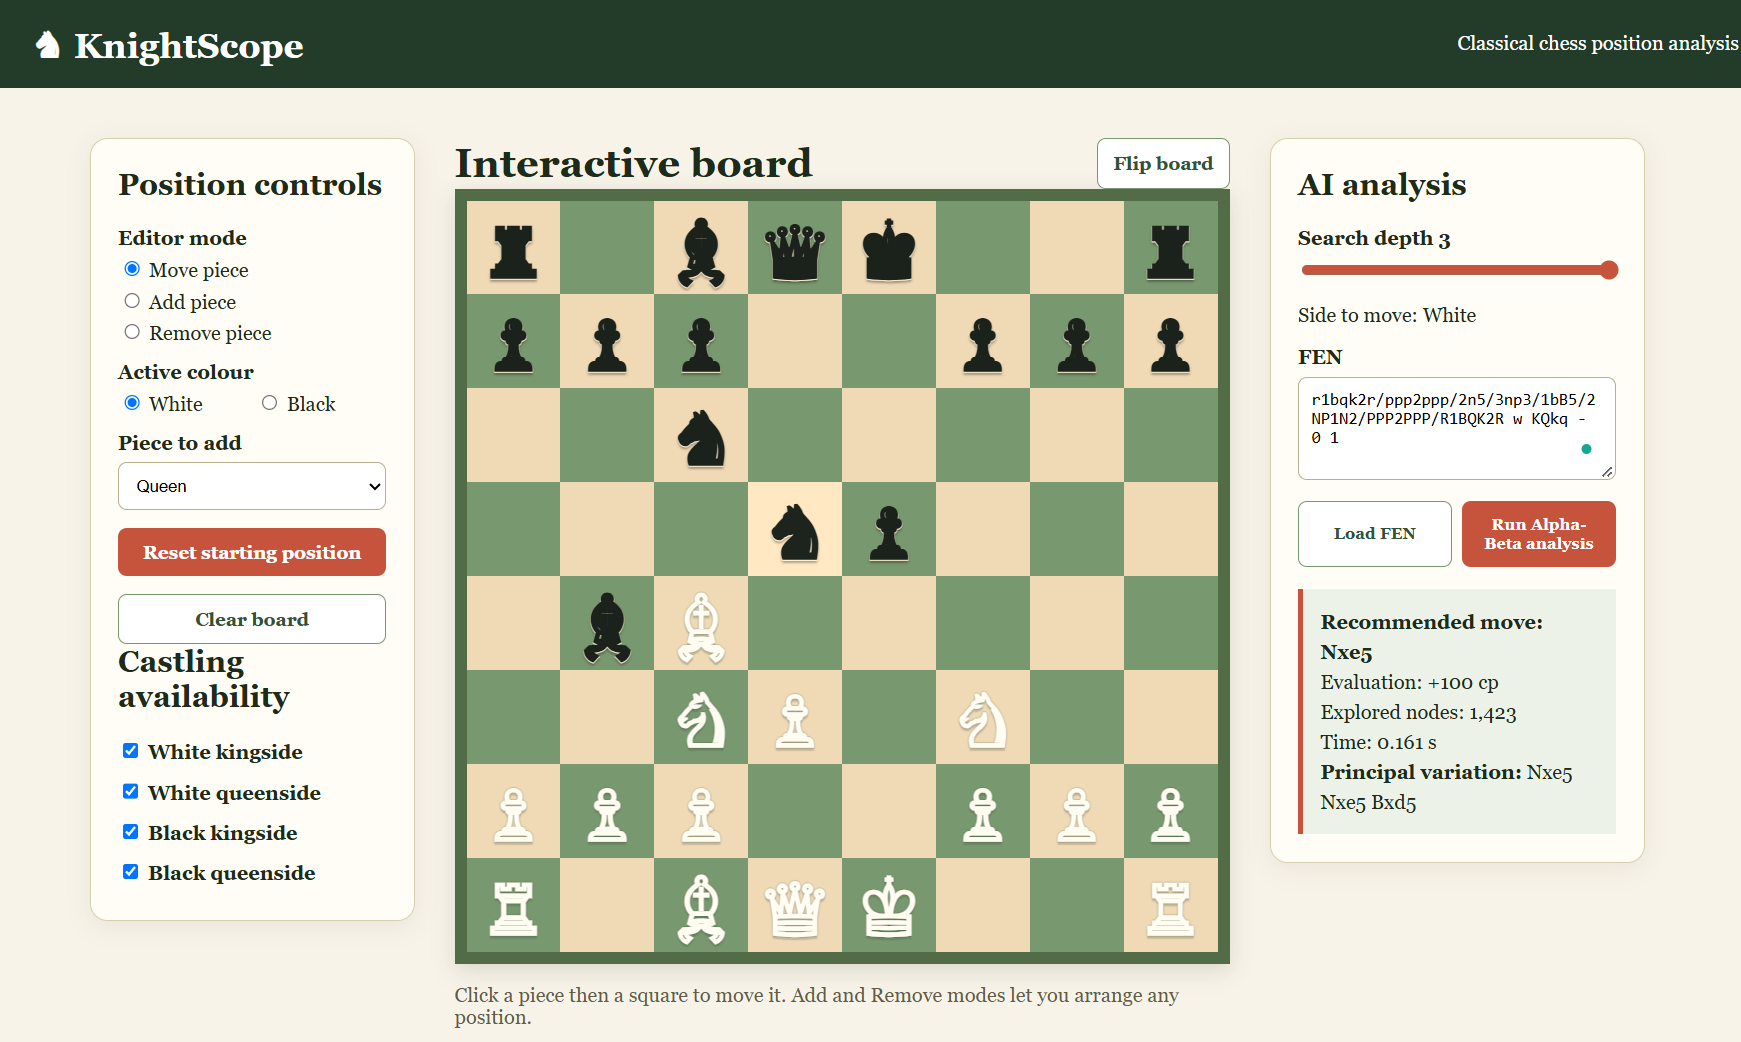
\includegraphics[width=0.92\textwidth]{images/tactical-depth3.png}
\caption{Depth-three tactical position: Nxe5, 1,423 explored nodes, and 0.161 seconds}\end{figure}
\begin{figure}[H]\centering
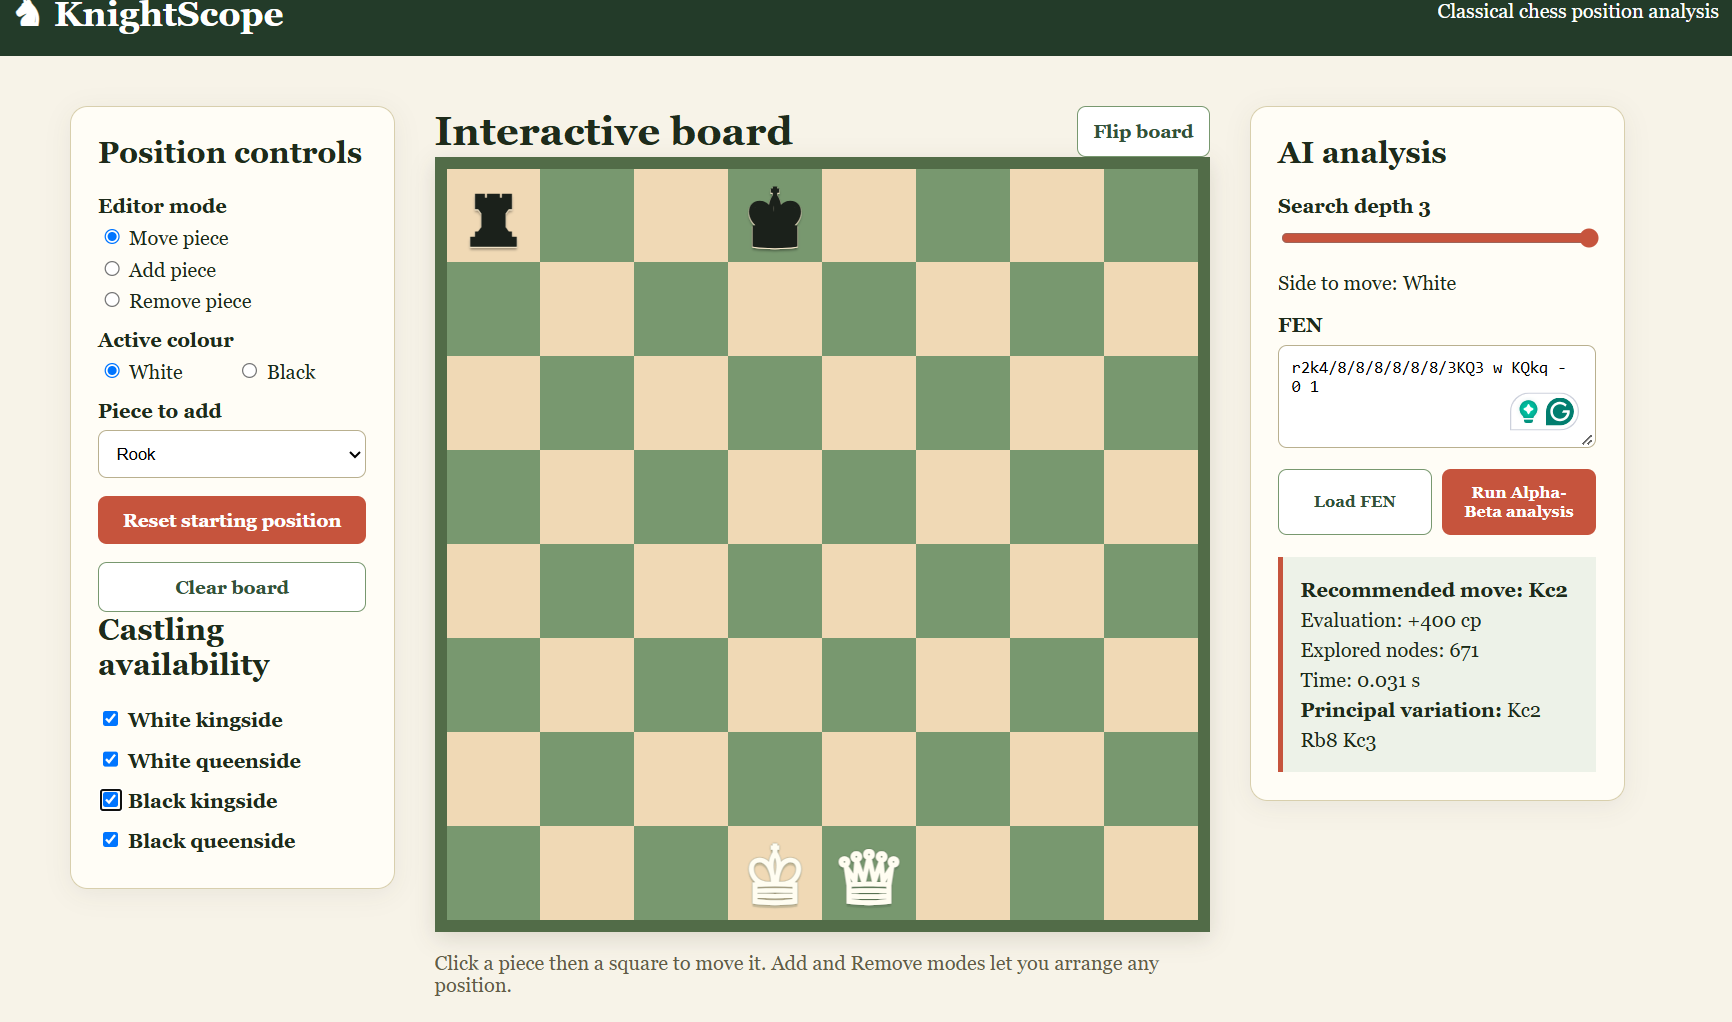
\includegraphics[width=0.92\textwidth]{images/custom-position.png}
\caption{Custom sparse position: Kc2, 671 explored nodes, and 0.031 seconds}\end{figure}

\chapter{Experimental Method}
The stored experiments use ten legal positions covering opening, tactical, defensive, checkmate, endgame, and middlegame cases. For Minimax and Alpha-Beta, the benchmark compares depths one through three. The timing procedure runs a search three times and reports the median duration. Each result records best move, score, explored nodes, pruned sibling moves, execution time, and nodes per second.

\begin{enumerate}[label=E\arabic*.]
\item Minimax versus Alpha-Beta: move and score equivalence, node reduction, and speed-up.
\item Search-depth scaling: Alpha-Beta nodes and time at deeper limits.
\item Greedy versus depth-three adversarial search: move agreement and tactical divergence.
\item Iterative Deepening: completed depth and measured runtime under several requested budgets.
\end{enumerate}
Timing figures are comparative observations from the stored run, not universal hardware guarantees.

\chapter{Results and Discussion}
\section{Minimax and Alpha-Beta}
Table~\ref{tab:ab} aggregates the 30 recorded comparisons. Alpha-Beta returned the same move and score as Minimax at every recorded depth. Pruning has no effect at depth one because there is no interior branch to cut off. The benefit becomes substantial at deeper searches.
\begin{table}[H]\centering\caption{Recorded Alpha-Beta comparison across ten positions}\label{tab:ab}
\begin{tabular}{ccccccc}\toprule
Depth & Cases & Score match & Move match & Mean reduction & Range & Mean speed-up\\\midrule
1 & 10 & 10/10 & 10/10 & 0.00\% & 0.00--0.00\% & 1.01$\times$\\
2 & 10 & 10/10 & 10/10 & 82.16\% & 60.67--93.01\% & 9.29$\times$\\
3 & 10 & 10/10 & 10/10 & 94.11\% & 78.74--98.87\% & 29.31$\times$\\\bottomrule
\end{tabular}\end{table}
\begin{figure}[H]\centering
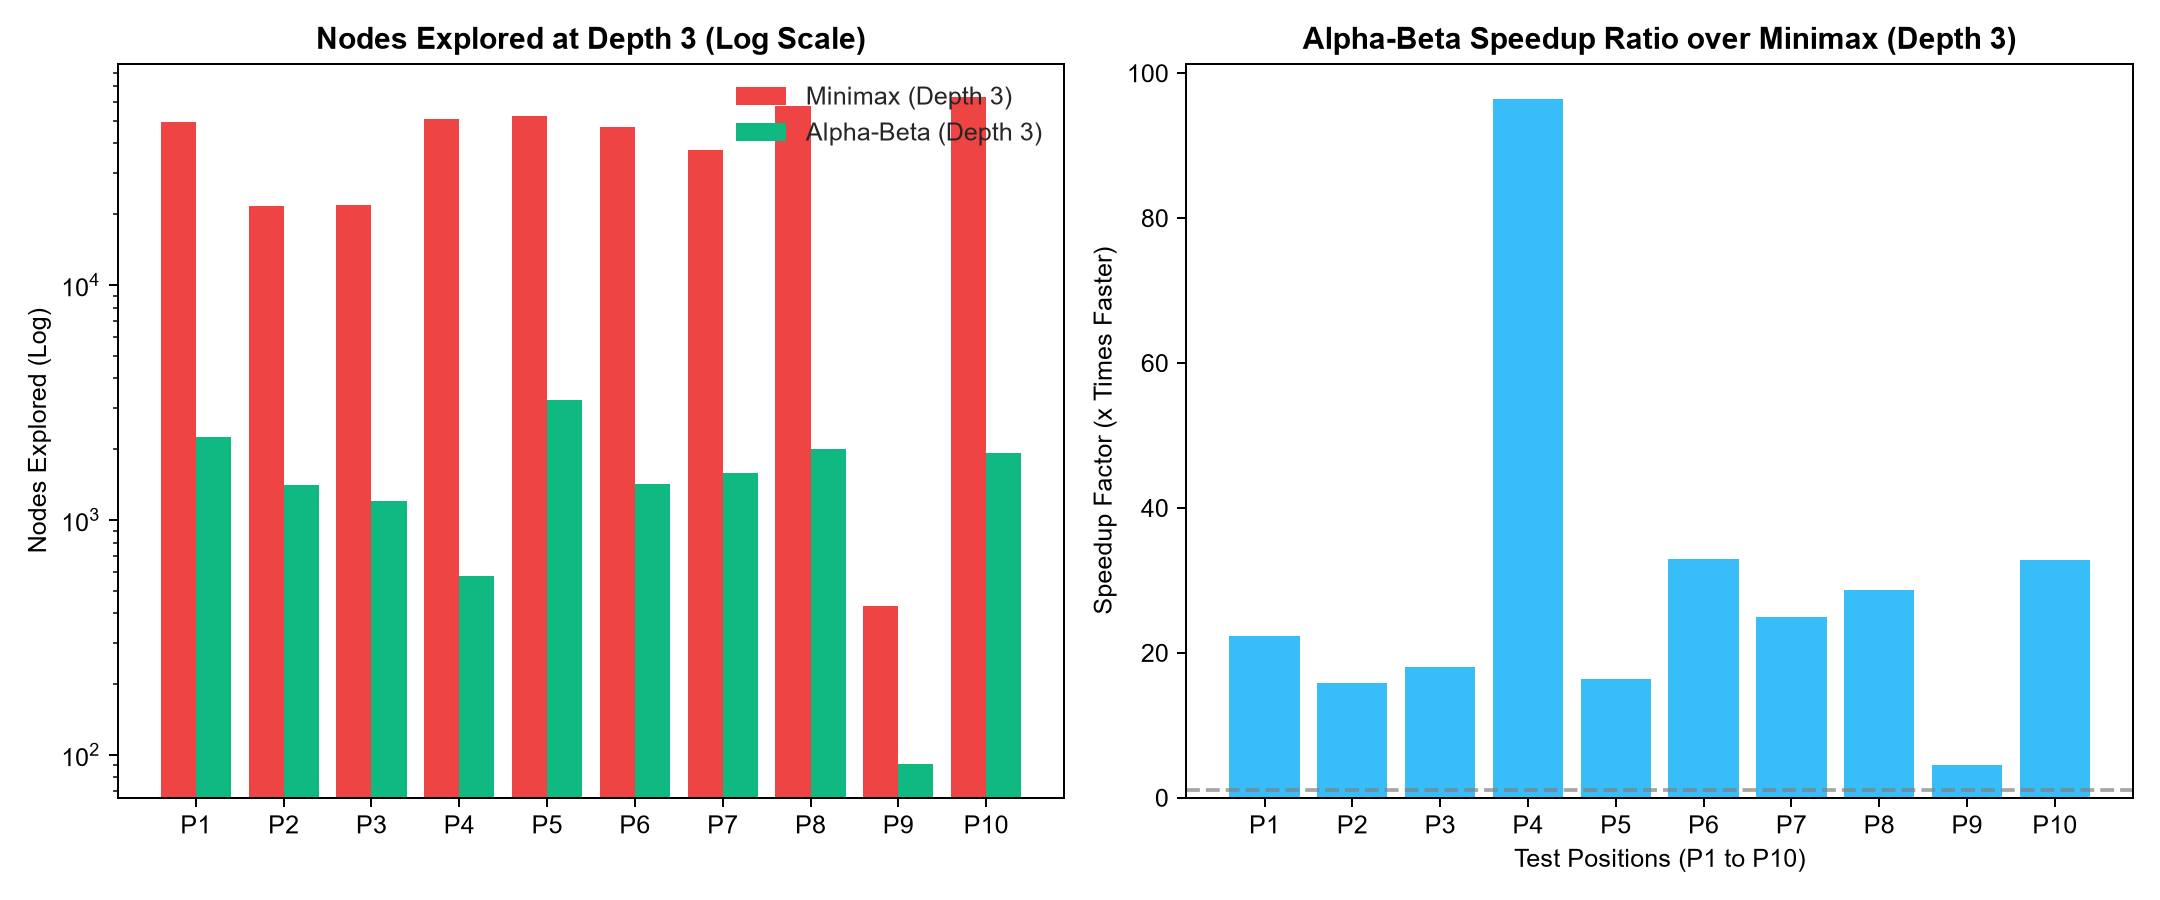
\includegraphics[width=0.88\textwidth]{images/minimax_vs_alphabeta_chart.png}
\caption{Stored benchmark chart comparing Minimax and Alpha-Beta}\end{figure}

\section{Greedy Baseline}
Greedy's immediate move agrees with the depth-three Alpha-Beta choice in 2 of 10 recorded positions: a forced-mate position and an endgame. It selects a different move in the other 8 positions. This supports the intended lesson that immediate heuristic improvement does not substitute for modelling an opponent's best reply. It does not prove that every Greedy choice loses material or is objectively losing.
\begin{table}[H]\centering\caption{Greedy and depth-three adversarial moves}\small
\begin{tabular}{cccc}\toprule Position & Greedy & Alpha-Beta depth 3 & Agreement\\\midrule
pos\_01 & Nxe4 & Bb4 & No\\pos\_02 & Nxe5 & Bb5 & No\\pos\_03 & Nxe5 & Bb5 & No\\pos\_04 & Bxd5 & Nxe5 & No\\pos\_05 & Nxe5 & Bd5 & No\\pos\_06 & Qxf7\# & Qxf7\# & Yes\\pos\_07 & Nxe4 & Bc5 & No\\pos\_08 & Bxh7 & Bb5 & No\\pos\_09 & Kd3 & Kd3 & Yes\\pos\_10 & Nxc6 & Bb5 & No\\\bottomrule
\end{tabular}\end{table}

\section{Iterative Deepening Measurements}
The stored experiment requested budgets from 0.2 to 2.0 seconds. A shallow valid result is recorded before a deeper attempt, but a complete iteration may exceed the requested budget because the underlying Alpha-Beta call is not interruptible. The maximum recorded actual runtimes were 1.74, 12.30, 12.58, and 12.45 seconds for the four requested budgets. The data demonstrates progressive-depth behaviour but does not validate strict real-time compliance.

\chapter{Verification and Testing}
The repository includes test modules for chess rules, FEN validation, terminal states, material evaluation, algorithm legality, Minimax/Alpha-Beta equivalence, Greedy node counts, Iterative Deepening progression, and benchmark-position validity. The source files parse successfully in the available validation environment. That environment did not include the project's Python dependencies, including \texttt{python-chess} and \texttt{pytest}, so this final review could not re-execute the test suite there. The report therefore distinguishes stored experiment outputs from newly reproduced outputs.

\chapter{Limitations and Future Work}\label{ch:limits}
\begin{enumerate}
\item \textbf{Depth horizon:} tactics beyond the selected depth may be missed. Quiescence search would help around captures and checks.
\item \textbf{Time-limit enforcement:} a deadline check inside Alpha-Beta should propagate a timeout and return the last fully completed result.
\item \textbf{No transposition table:} equivalent positions can be searched again through different move orders. Zobrist hashing and a transposition table would reduce repeated work.
\item \textbf{Handcrafted evaluation:} fixed weights omit strategic concepts and have not been calibrated against a human or engine corpus.
\item \textbf{Benchmark scope:} ten positions support a course demonstration, not general claims about all chess positions or hardware.
\end{enumerate}

\chapter{Conclusion}
KnightScope fulfils the course objective of applying classical AI to a practical game-analysis problem. It models legal chess positions as adversarial state spaces, implements four related search techniques, provides a visual interface, and includes benchmark artefacts. The saved results show Alpha-Beta returns the same depth-limited choices as Minimax while examining substantially fewer nodes at greater depths. Greedy frequently chooses a different move from depth-three adversarial search. The remaining limitations, especially strict time-limit enforcement, are stated as next steps rather than hidden by unsupported claims.

\chapter*{Team Contributions}\addcontentsline{toc}{chapter}{Team Contributions}
\begin{tabular}{p{0.18\textwidth}p{0.70\textwidth}}\toprule
Member 1 & Board representation, FEN processing, legal-move utilities, and integration.\\
Member 2 & Minimax and Alpha-Beta implementation.\\
Member 3 & Greedy, Iterative Deepening, and heuristic evaluation.\\
Member 4 & Streamlit interface, visualisation, benchmarking, and documentation.\\\bottomrule
\end{tabular}

\chapter*{References}\addcontentsline{toc}{chapter}{References}
\begin{enumerate}[label={[\arabic*]}]
\item S. Russell and P. Norvig, \textit{Artificial Intelligence: A Modern Approach}, 4th ed., Pearson, 2020.
\item C. E. Shannon, ``Programming a Computer for Playing Chess,'' \textit{Philosophical Magazine}, vol. 41, no. 314, pp. 256--275, 1950.
\item D. E. Knuth and R. W. Moore, ``An Analysis of Alpha-Beta Pruning,'' \textit{Artificial Intelligence}, vol. 6, no. 4, pp. 293--326, 1975.
\item R. E. Korf, ``Depth-first Iterative-Deepening: An Optimal Admissible Tree Search,'' \textit{Artificial Intelligence}, vol. 27, no. 1, pp. 97--109, 1985.
\item python-chess documentation, \url{https://python-chess.readthedocs.io/}.
\item KnightScope source repository, \url{https://github.com/HaMaMi-1/KnightScope}.
\item KnightScope public demonstration, \url{https://knightscope-classic.onrender.com}.
\end{enumerate}
\appendix
\chapter{Reproducibility Guide}
Install requirements with \texttt{pip install -r requirements.txt}. Run tests with \texttt{pytest -q}. Regenerate experiment CSV files with \texttt{python -m analysis.experiments}. Open the public demonstration at \url{https://knightscope-classic.onrender.com}. Timing results vary by CPU, package versions, and background load.
\chapter{Selected Search Pseudocode}
\begin{lstlisting}
function ALPHABETA(state, depth, alpha, beta):
    if terminal(state) or depth == 0: return evaluate(state)
    for move in ordered_legal_moves(state):
        value = ALPHABETA(result(state, move), depth - 1, alpha, beta)
        update alpha at MAX or beta at MIN
        if beta <= alpha: stop exploring sibling moves
    return best value and principal variation
\end{lstlisting}
\end{document}
